\documentclass[journal,10pt]{IEEEtran}
% ---------------------------------------------------------------------------
% Ranking Is Not the Problem: Leakage-Free Benchmarking of Sentiment Classifiers on Twitter and IMDB. Build: python paper/build.py  (PDF via tectonic,
% DOCX via pandoc). Every table in tables/ and the architecture figure are
% generated by paper/make_tables.py from reports/results.csv and the model
% cards; no number in this manuscript is typed by hand.
% ---------------------------------------------------------------------------
\usepackage[utf8]{inputenc}
\usepackage[T1]{fontenc}
\usepackage{graphicx}
\usepackage{booktabs}
\usepackage{amsmath,amssymb}
\usepackage{multirow}
\usepackage[hyphens]{url}
\usepackage{textcomp}
\usepackage{microtype}
\usepackage[hidelinks]{hyperref}
\graphicspath{{figures/}{../reports/figures/}}
\def\UrlBreaks{\do\/\do-\do.}
% IEEEtran prints "Abstract---" and "Index Terms---"; use a colon instead
\usepackage{etoolbox}
\makeatletter
\patchcmd{\abstract}{\textit{\abstractname}---\relax}{\textit{\abstractname:}\ \relax}{}{\ClassWarning{paper}{abstract header not patched}}
\patchcmd{\IEEEkeywords}{\textit{\IEEEkeywordsname}---\relax}{\textit{\IEEEkeywordsname:}\ \relax}{}{\ClassWarning{paper}{keywords header not patched}}
\makeatother

\begin{document}

\IfFileExists{title.tex}{\input{title}}{\newcommand{\PaperTitle}{Ranking Is Not the Problem: Leakage-Free Benchmarking of Sentiment Classifiers on Twitter and IMDB}\newcommand{\PaperShortTitle}{Ranking Is Not the Problem}}
\title{\PaperTitle}

\author{Rakibul~Hasan~Sium\\
\normalsize Nanjing University of Information Science and Technology, Nanjing, China\\
\normalsize sium@nuist.edu.cn%
\thanks{Code, configuration, model cards and all figures: \url{https://github.com/rhs2/sentiment-ml-benchmark}.}}

\markboth{Sium: \PaperShortTitle}{Sium: \PaperShortTitle}

\maketitle

\begin{abstract}
Comparisons of sentiment classifiers on social-media text often differ in evaluation practice more than in modelling: vectorizers fitted on test data, a fixed decision threshold, or accuracy reported on heavily imbalanced classes can move a result by more than the difference between methods. We present a benchmark of eight model families (multinomial naive Bayes, logistic regression, a calibrated linear support vector machine, random forest, gradient-boosted trees, a soft-voting ensemble, a convolutional network and a bidirectional LSTM) across five input representations (count and TF-IDF $n$-grams, mean-pooled Word2Vec, Doc2Vec and token sequences) on three corpora: racist and sexist tweet detection (31,962 tweets, 7\,percent positive), COVID-19 vaccine tweets with lexicon-derived labels (10,353 tweets, three classes) and the IMDB movie-review corpus (50,000 reviews). Every cell of the 56-cell grid follows one protocol: stratified cross-validation on the training split yields out-of-fold probabilities, from which the decision threshold and the model are selected; the test split is scored once. On the hate-speech task all families reach ROC-AUC between 0.939 and 0.952, while F1 on the positive class ranges from 0.608 to 0.684 depending on calibration and threshold transfer, not on ranking ability; tuning the threshold on out-of-fold predictions adds up to 0.09 F1 for the classical models and 0.14 for the networks over the default of 0.5. On the vaccine task the CNN reaches macro F1 0.812 against 0.775 for the best classical model, and on IMDB the linear $n$-gram models (F1 0.884 to 0.888, accuracy 0.882 to 0.885) form the ceiling of the grid, matching published results for models without pretrained language representations. Learned document embeddings are the weakest representation on every task. The benchmark is released as a maintained system with experiment tracking, model cards, a prediction service backed by PostgreSQL, population-stability drift monitoring and infrastructure definitions for cloud deployment, so that the reported numbers can be regenerated with one command and the selected models operated after publication.
\end{abstract}

\begin{IEEEkeywords}
Sentiment analysis, hate speech detection, text classification, evaluation methodology, calibration, threshold selection, reproducibility, MLOps.
\end{IEEEkeywords}

\section{Introduction}
\IEEEPARstart{S}{entiment} classification of short social-media text is one of the most frequently reported tasks in applied natural language processing, and comparisons of classical learners with neural networks on Twitter data are abundant~\cite{pang2008,liu2012}. Such comparisons are, however, sensitive to evaluation choices that are rarely controlled. Fitting a vocabulary or an embedding model on the union of training and test data leaks test information into the features~\cite{kaufman2012}; selecting a model on the same split that is reported overstates its score~\cite{cawley2010}; reporting accuracy on a task with 7\,percent positives rewards the majority class; and evaluating probabilistic classifiers at a fixed decision threshold conflates the quality of the ranking they produce with the calibration of their scores~\cite{lipton2014,guo2017}. Each of these effects can exceed the differences between methods that papers then rank.

This article grew out of the author's undergraduate thesis, which compared naive Bayes, logistic regression, a support vector machine, a random forest and gradient-boosted trees on two Twitter corpora in notebook form, with exactly the shortcomings listed above. We re-implement that study as a benchmark in which the evaluation protocol is fixed once and applied to every combination of dataset, representation and model, extend it with the neural models that the thesis proposed as future work and with a third, balanced corpus of long documents, and ship it as a maintained system rather than as a set of scripts. The contributions are:

\begin{enumerate}
\item A 56-cell benchmark (three corpora, five representations, eight model families) under one leakage-free protocol: features fitted per cross-validation fold, decision thresholds chosen on out-of-fold predictions, model selection by cross-validated F1, and a single scoring pass on a held-out split (Section~\ref{sec:method}).
\item An analysis that separates ranking ability from thresholding and calibration. On the imbalanced hate-speech task all eight families are within 0.013 ROC-AUC of each other, yet their positive-class F1 spans 0.076, and the family with the best cross-validated F1 transfers its threshold worst (Section~\ref{sec:results}).
\item Evidence across the three corpora that sparse $n$-gram features remain the strongest representation for classical learners on short text, that learned document embeddings are the weakest representation on every task, and that on balanced long documents linear models on TF-IDF match networks trained from scratch at a fraction of the cost.
\item A reference implementation in which every number in this paper is regenerated from the saved out-of-fold and test probabilities, each run is tracked, the selected model is exported with a model card~\cite{mitchell2019} and a monitoring baseline, and a prediction service with database-backed drift detection turns the benchmark into an operable system~\cite{sculley2015}.
\end{enumerate}

\section{Related Work}
Sentiment analysis and opinion mining are surveyed by Pang and Lee~\cite{pang2008} and Liu~\cite{liu2012}. For Twitter specifically, Go et al.~\cite{go2009} introduced distant supervision with emoticons as noisy labels, a precursor of the lexicon-derived labels used in our vaccine corpus, and Waseem and Hovy~\cite{waseem2016} and Davidson et al.~\cite{davidson2017} established racist and sexist tweet detection as a task with strong class imbalance, in which F1 on the minority class is the metric of interest. Classical text classifiers remain competitive baselines: multinomial naive Bayes~\cite{mccallum1998}, linear support vector machines~\cite{joachims1998}, random forests~\cite{breiman2001} and gradient boosting~\cite{chen2016}. Wang and Manning~\cite{wang2012} showed that linear models over bigram features are hard to beat on sentiment corpora such as IMDB~\cite{maas2011}, which is consistent with our IMDB results. Distributed representations for text, Word2Vec~\cite{mikolov2013} and Doc2Vec~\cite{le2014}, and the two neural architectures we include, the text CNN of Kim~\cite{kim2014} and the LSTM~\cite{hochreiter1997}, are standard. Pretrained transformers~\cite{devlin2019} set the current ceiling on these corpora; we deliberately restrict the grid to models that train from scratch on a CPU and quantify the remaining gap.

On methodology, Kaufman et al.~\cite{kaufman2012} catalogue leakage, Cawley and Talbot~\cite{cawley2010} show how model selection on the evaluation data biases reported scores, Lipton et al.~\cite{lipton2014} prove that the F1-optimal threshold depends on the classifier and the class prior, and Platt~\cite{platt1999}, Niculescu-Mizil and Caruana~\cite{niculescu2005} and Guo et al.~\cite{guo2017} study the calibration of margin-based and neural classifiers; Davis and Goadrich~\cite{davis2006} motivate precision-recall analysis under imbalance. On the systems side, Sculley et al.~\cite{sculley2015} describe the operational debt of machine learning, Mitchell et al.~\cite{mitchell2019} propose model cards, and MLflow~\cite{zaharia2018} provides experiment tracking; population stability indices for drift originate in credit scoring~\cite{siddiqi2006}.

\section{Datasets}
\label{sec:data}
Table~\ref{tab:data} summarises the corpora. The first two are the thesis experiments; the third is an addition chosen to contrast short, imbalanced social-media text with long, balanced reviews.

\begin{table}[t]
\centering
\caption{Corpora. Splits are stratified 80/20 holdouts with a fixed seed for the Twitter corpora and the official split for IMDB.}
\label{tab:data}
\footnotesize\setlength{\tabcolsep}{4pt}
\begin{tabular}{lrll}
\toprule
Corpus & Docs & Classes & Labels \\
\midrule
Hate (Twitter) & 31,962 & 2; 7.0\,\% positive & human (competition) \\
Vaccine (Twitter) & 10,353 & 3; 9.9 / 56.6 / 33.5\,\% & lexicon polarity \\
IMDB & 50,000 & 2; balanced & human (ratings) \\
\bottomrule
\end{tabular}
\end{table}

\textbf{Hate.} The Analytics Vidhya Twitter sentiment practice set: 31,962 tweets labelled 1 when racist or sexist, 0 otherwise (2,242 positives). Handles are anonymised as \texttt{@user} in the source; the competition's unlabelled test file is not used. We split stratified 80/20 (seed 42), giving 25,569 training and 6,393 test tweets.

\textbf{Vaccine.} Pfizer and BioNTech COVID-19 vaccine tweets from Kaggle (11,020 rows). As in the thesis, no human labels exist: after light cleaning and de-duplication (10,353 unique tweets), each tweet is labelled by the sign of its TextBlob~\cite{loria2018} polarity as negative, neutral or positive. Scores on this corpus therefore measure agreement with a lexicon labeller rather than with human judgement; we keep it because it is half of the original study and because it exposes how representations interact with lexicon-defined targets.

\textbf{IMDB.} The Large Movie Review Dataset of Maas et al.~\cite{maas2011}: 25,000 training and 25,000 test reviews, balanced, with negative defined as a rating of at most 4 and positive as at least 7. We use the official split.

No corpus is redistributed with the code. Download locations are read from the environment, and a manifest records the SHA-256 hash, row count and class balance of the files used for a run, together with a content fingerprint of the loaded frame that is written into every model card.

\section{Methodology}
\label{sec:method}

\subsection{Text normalisation}
One transformer implements the thesis recipe and is the first step of every exported pipeline, so training, evaluation and serving apply identical cleaning: HTML unescape and tag removal, lower-casing, removal of URLs and @-handles, retention of letters only (hashtags optionally kept as tokens), a minimum token length, the scikit-learn English stop-word list, and Porter stemming. The hate corpus keeps hashtags and drops tokens shorter than three characters; the vaccine and IMDB corpora drop the hash symbol and keep two-character tokens.

\subsection{Representations}
Five representations are evaluated. \emph{Counts} and \emph{TF-IDF} use unigrams and bigrams with document-frequency bounds (minimum 2, maximum 90\,percent), a 5,000-term vocabulary for tweets and 20,000 terms for reviews, and sublinear term frequency for TF-IDF. \emph{Word2Vec}~\cite{mikolov2013} is a skip-gram model (200 dimensions, window 5, 10 negative samples, 20 epochs on tweets and 8 on reviews) trained on the training fold only, with the document vector as the mean of its token vectors. \emph{Doc2Vec}~\cite{le2014} is a distributed-memory model (200 dimensions, 15 epochs) in which both training and test documents are embedded by inference, so that the two are represented the same way. \emph{Sequence} denotes padded token identifiers (vocabulary of at most 20,000 tokens for tweets, 30,000 for reviews; 48 tokens for tweets, 200 for the CNN and 160 for the BiLSTM on reviews) consumed by the neural models, whose embedding layer is initialised from a Word2Vec model trained on the same fold.

\subsection{Models}
Classical models use scikit-learn~\cite{pedregosa2011} and XGBoost~\cite{chen2016}: multinomial naive Bayes (additive smoothing 0.5, count-based features only), logistic regression (L2, $C{=}1$ on tweets and 2 on reviews, balanced class weights on the Twitter corpora), a linear SVM wrapped in sigmoid calibration with three internal folds~\cite{platt1999} so that it exposes probabilities, a random forest (400 trees, balanced subsample weights; 300 trees on IMDB), gradient-boosted trees (histogram method, depth 6, 500 rounds at learning rate 0.05 on tweets; 400 rounds at 0.1 on reviews, subsample 0.9, column subsample 0.5), and a soft-voting ensemble of the logistic regression, the calibrated SVM and XGBoost with equal weights. The thesis' boosted-tree parameters (depth 8, minimum child weight 6, $\gamma{=}1.2$) were tuned on Word2Vec features and under-fit sparse $n$-gram matrices; they are retained in the configuration for reference but not used.

The neural models are implemented in PyTorch~\cite{paszke2019} and wrapped as scikit-learn estimators so that they pass through the same cross-validation, threshold selection, tracking and export as the classical models. The CNN follows Kim~\cite{kim2014}: 128-dimensional embeddings, kernel widths 3, 4 and 5 with 128 filters each, global max pooling, dropout 0.5. The BiLSTM~\cite{hochreiter1997} has 128 hidden units per direction (64 on reviews) with concatenated max and mean pooling over time. Both train with Adam (learning rate $10^{-3}$), batch size 64, a class-weighted cross-entropy on the imbalanced corpora, and early stopping on a 10\,percent validation slice of the training fold (at most eight epochs on tweets, four and three on reviews).

\subsection{Evaluation protocol}
\label{sec:protocol}
The same procedure is applied to every (corpus, representation, model) cell:
\begin{enumerate}
\item The training split is cleaned once. Each representation is fitted once per cross-validation fold on that fold's training part and once on the whole training split; the resulting matrices are cached and shared by all models evaluated on that representation, so that models are compared on identical inputs and no representation ever sees validation or test documents during fitting.
\item Stratified $k$-fold cross-validation ($k{=}5$ on tweets, $3$ on reviews) produces out-of-fold class probabilities for every training document.
\item For binary tasks, the decision threshold on $P(\text{positive})$ is the value in $[0.05, 0.95]$ that maximises F1 on the out-of-fold probabilities~\cite{lipton2014}. The three-class task uses the arg-max.
\item The selected cell per corpus is the one with the highest cross-validated F1 at that threshold; the test split plays no part in selection~\cite{cawley2010}.
\item The model is refitted on the whole training split and scored once on the test split at the selected threshold: accuracy, precision, recall, F1 (positive class, or macro average), ROC-AUC, average precision, a per-class report and a confusion matrix. F1 at the default threshold of 0.5 is recorded alongside.
\item Out-of-fold and test probabilities are saved, so that every figure and table is regenerated from disk without retraining.
\end{enumerate}
F1 on the positive class is the primary metric on the hate corpus because accuracy is dominated by the 93\,percent majority class; macro F1 is used on the three-class corpus; both F1 and accuracy are reported on the balanced IMDB corpus.

\subsection{System}
Fig.~\ref{fig:arch} shows the implementation. One YAML file defines a benchmark (datasets, cleaning, representations, models, grid, folds, seed) and is logged with every run; each cell is an MLflow~\cite{zaharia2018} run with parameters, cross-validated and test metrics, the threshold, timings and the confusion matrix, and the selected pipeline per corpus is exported as one serialised object (cleaner, representation, model) together with a model card~\cite{mitchell2019} (data fingerprint, selection rule, metrics, per-class scores, software versions, commit) and a monitoring baseline. A Flask service exposes prediction, health and statistics endpoints over the exported pipelines and writes every prediction to a PostgreSQL store; a monitor compares recent traffic with the training baseline using the population stability index~\cite{siddiqi2006} of the token-length and predicted-class distributions, the out-of-vocabulary rate against the training vocabulary, and the share of inputs that become empty after cleaning, with warning and alert levels and a stored history. Continuous integration runs the unit tests against PostgreSQL, a one-minute version of the benchmark on a synthetic corpus, and a container build on every change; infrastructure definitions provision a container service, a managed database, object storage for artifacts and a scheduled drift task on a public cloud. No credential or dataset location appears in the code.

\begin{figure}[t]
\centering
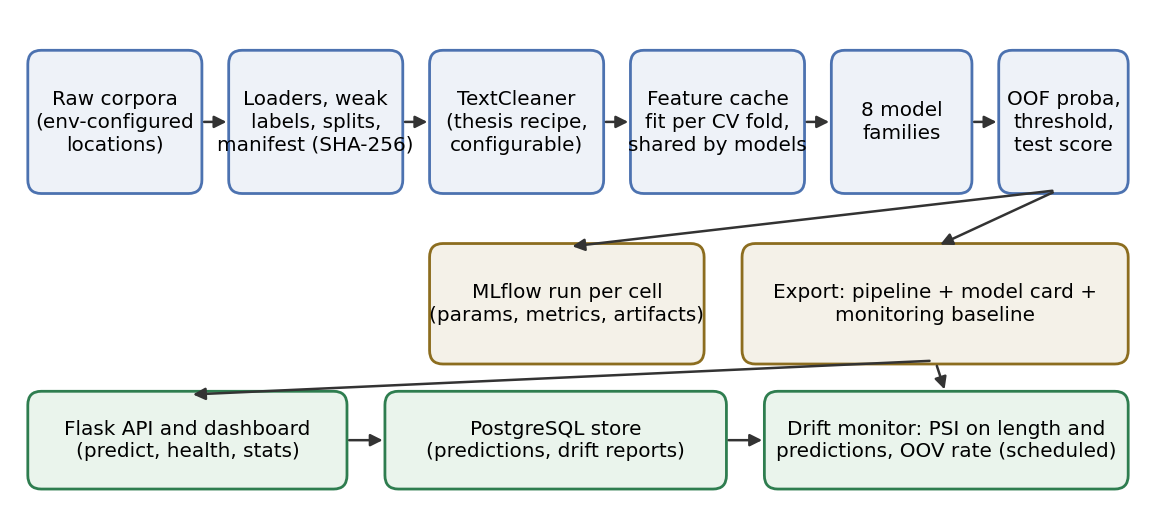
\includegraphics[width=\columnwidth]{architecture.png}
\caption{From configuration to operation: the benchmark (top), tracking and export (middle), and the prediction service with database-backed drift monitoring (bottom).}
\label{fig:arch}
\end{figure}

\section{Experimental Setup}
All results were produced on a laptop CPU (eight cores, no GPU) with pinned package versions (scikit-learn 1.5, XGBoost 2.0, Gensim 4.4, PyTorch 2.13). Seeds are fixed for the split, the folds, Gensim and PyTorch; Gensim's multithreaded training introduces run-to-run variation of the order of $10^{-3}$ in F1 for the embedding-based cells. The Twitter grid comprises 22 cells per corpus (naive Bayes on count-based features only, the ensemble on TF-IDF and Word2Vec, the networks on sequences); the IMDB grid is reduced to 12 cells for cost (no Doc2Vec, the random forest and SVM on TF-IDF only, shorter network schedules). The whole study runs in about two hours.

\section{Results}
\label{sec:results}
Table~\ref{tab:selected} lists the selected model per corpus, Table~\ref{tab:families} every family at its best representation, and Table~\ref{tab:features} every representation at its best model. Figures~\ref{fig:roc} to~\ref{fig:cv} are drawn from the saved probabilities of the hate corpus, the task on which evaluation choices matter most.

\begin{table*}[t]
\centering
\caption{Model selected per dataset by cross-validated F1, scored once on the held-out test split. F1 is on the positive class for the binary tasks and macro-averaged for the three-class task; ROC-AUC for the three-class task is one-versus-rest, macro-averaged. Thresholds are chosen on out-of-fold predictions (argmax for the three-class task).}
\label{tab:selected}
\footnotesize\setlength{\tabcolsep}{4pt}
\begin{tabular}{llrrlccccccc}
\toprule
Dataset & Task & Train & Test & Model / features & CV F1 & Test F1 & Acc. & Prec. & Rec. & ROC-AUC & Thr. \\
\midrule
Hate & binary & 25569 & 6393 & CNN / sequence & 0.672 \textpm\  0.022 & \textbf{0.608} & 0.955 & 0.782 & 0.498 & 0.948 & 0.90 \\
Vaccine & multiclass & 8282 & 2071 & CNN / sequence & 0.799 \textpm\  0.012 & \textbf{0.812} & 0.859 & 0.798 & 0.830 & 0.948 & argmax \\
IMDB & binary & 25000 & 25000 & Linear SVM (calib.) / TF-IDF & 0.893 \textpm\  0.002 & \textbf{0.884} & 0.882 & 0.870 & 0.898 & 0.953 & 0.50 \\
\bottomrule
\end{tabular}
\end{table*}
\begin{table*}[t]
\centering
\caption{Every model family at its best feature set per dataset (feature set chosen by cross-validated F1). Cells give test F1 with the cross-validated mean \textpm{} standard deviation across folds underneath. The best test F1 per column is in bold.}
\label{tab:families}
\begin{tabular}{llll}
\toprule
Model & Hate & Vaccine & IMDB \\
\midrule
Naive Bayes & \begin{tabular}[t]{@{}l@{}}0.658 (TF-IDF) \\ \scriptsize CV 0.650 \textpm\  0.017\end{tabular} & \begin{tabular}[t]{@{}l@{}}0.698 (counts) \\ \scriptsize CV 0.681 \textpm\  0.011\end{tabular} & \begin{tabular}[t]{@{}l@{}}0.851 (TF-IDF) \\ \scriptsize CV 0.868 \textpm\  0.002\end{tabular} \\
Logistic regression & \begin{tabular}[t]{@{}l@{}}0.654 (TF-IDF) \\ \scriptsize CV 0.652 \textpm\  0.009\end{tabular} & \begin{tabular}[t]{@{}l@{}}0.775 (counts) \\ \scriptsize CV 0.769 \textpm\  0.014\end{tabular} & \begin{tabular}[t]{@{}l@{}}0.886 (TF-IDF) \\ \scriptsize CV 0.892 \textpm\  0.002\end{tabular} \\
Linear SVM (calib.) & \begin{tabular}[t]{@{}l@{}}0.654 (TF-IDF) \\ \scriptsize CV 0.654 \textpm\  0.012\end{tabular} & \begin{tabular}[t]{@{}l@{}}0.744 (counts) \\ \scriptsize CV 0.739 \textpm\  0.013\end{tabular} & \begin{tabular}[t]{@{}l@{}}0.884 (TF-IDF) \\ \scriptsize CV 0.893 \textpm\  0.002\end{tabular} \\
Random forest & \begin{tabular}[t]{@{}l@{}}0.680 (TF-IDF) \\ \scriptsize CV 0.669 \textpm\  0.021\end{tabular} & \begin{tabular}[t]{@{}l@{}}0.709 (counts) \\ \scriptsize CV 0.717 \textpm\  0.013\end{tabular} & \begin{tabular}[t]{@{}l@{}}0.859 (TF-IDF) \\ \scriptsize CV 0.859 \textpm\  0.002\end{tabular} \\
XGBoost & \begin{tabular}[t]{@{}l@{}}\textbf{0.684} (Word2Vec) \\ \scriptsize CV 0.664 \textpm\  0.020\end{tabular} & \begin{tabular}[t]{@{}l@{}}0.757 (counts) \\ \scriptsize CV 0.745 \textpm\  0.023\end{tabular} & \begin{tabular}[t]{@{}l@{}}0.865 (TF-IDF) \\ \scriptsize CV 0.862 \textpm\  0.003\end{tabular} \\
Soft-voting ensemble & \begin{tabular}[t]{@{}l@{}}0.662 (TF-IDF) \\ \scriptsize CV 0.659 \textpm\  0.013\end{tabular} & \begin{tabular}[t]{@{}l@{}}0.757 (TF-IDF) \\ \scriptsize CV 0.754 \textpm\  0.014\end{tabular} & \begin{tabular}[t]{@{}l@{}}\textbf{0.888} (TF-IDF) \\ \scriptsize CV 0.891 \textpm\  0.002\end{tabular} \\
CNN & \begin{tabular}[t]{@{}l@{}}0.608 (sequence) \\ \scriptsize CV 0.672 \textpm\  0.022\end{tabular} & \begin{tabular}[t]{@{}l@{}}\textbf{0.812} (sequence) \\ \scriptsize CV 0.799 \textpm\  0.012\end{tabular} & \begin{tabular}[t]{@{}l@{}}0.875 (sequence) \\ \scriptsize CV 0.872 \textpm\  0.003\end{tabular} \\
BiLSTM & \begin{tabular}[t]{@{}l@{}}0.658 (sequence) \\ \scriptsize CV 0.670 \textpm\  0.018\end{tabular} & \begin{tabular}[t]{@{}l@{}}0.779 (sequence) \\ \scriptsize CV 0.731 \textpm\  0.029\end{tabular} & \begin{tabular}[t]{@{}l@{}}0.876 (sequence) \\ \scriptsize CV 0.879 \textpm\  0.000\end{tabular} \\
\bottomrule
\end{tabular}
\end{table*}

\subsection{Ranking ability versus thresholding}
On the hate corpus every family reaches a test ROC-AUC between 0.939 (calibrated SVM) and 0.952 (XGBoost on Word2Vec), and average precision between 0.695 and 0.762 (Fig.~\ref{fig:roc}); the eight families order the test tweets almost equally well. Their F1 on the positive class, however, spans 0.608 to 0.684, and the spread is explained by calibration and threshold transfer rather than by ranking. Fig.~\ref{fig:calib} shows that the class-weighted networks are strongly over-confident (mean predicted probability 0.87 in the top decile against an observed positive rate of 0.51), whereas the calibrated SVM, the forest, the boosted trees and the ensemble lie close to the diagonal; accordingly the networks' F1-optimal thresholds are 0.85 and 0.90 (Fig.~\ref{fig:thr}) while the classical models' lie between 0.23 and 0.69.

\begin{figure}[t]
\centering
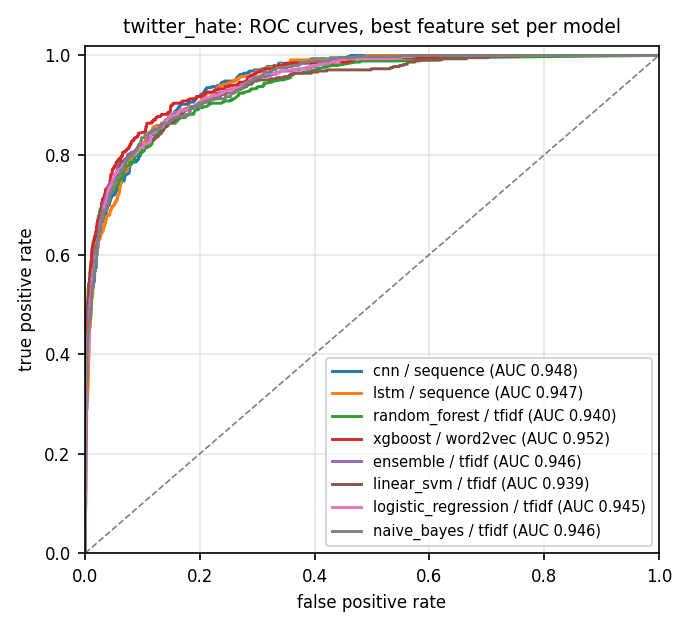
\includegraphics[width=\columnwidth]{roc_twitter_hate.png}
\caption{Hate corpus: ROC curves of the best representation per model family on the test split.}
\label{fig:roc}
\end{figure}

\begin{figure}[t]
\centering
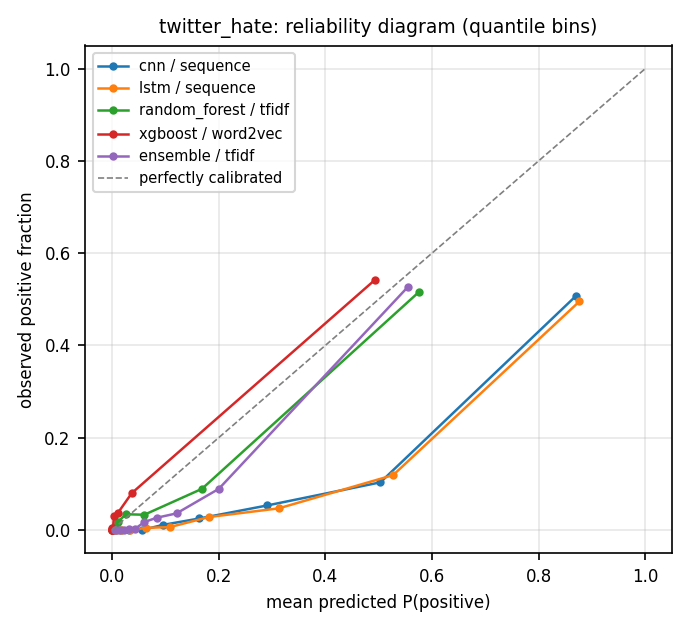
\includegraphics[width=\columnwidth]{calibration_twitter_hate.png}
\caption{Hate corpus: reliability diagram (quantile bins) of the five families with the highest cross-validated F1. The networks are over-confident; the tree and linear models are close to calibrated.}
\label{fig:calib}
\end{figure}

\begin{figure}[t]
\centering
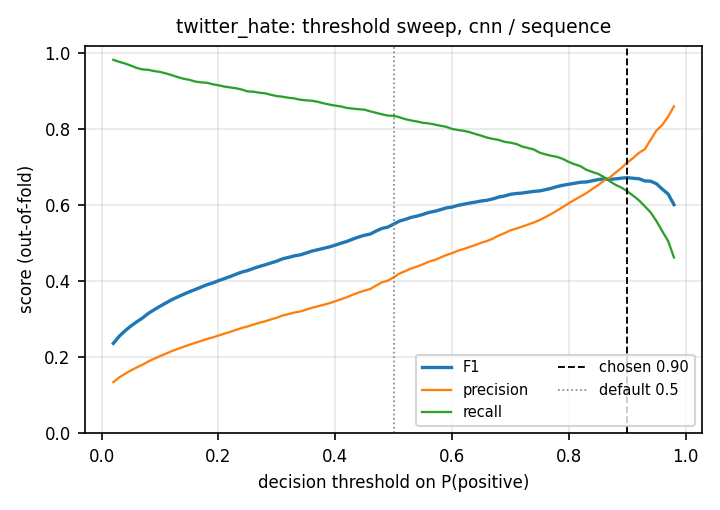
\includegraphics[width=\columnwidth]{threshold_twitter_hate.png}
\caption{Hate corpus: F1, precision and recall of the CNN as a function of the decision threshold on out-of-fold predictions. The F1 optimum lies at 0.90; the default of 0.5 gives recall 0.84 at precision 0.41.}
\label{fig:thr}
\end{figure}

\begin{table}[t]
\centering
\caption{Effect of the decision threshold on the hate-speech task (best feature set per model). F1 at the threshold tuned on out-of-fold predictions versus F1 at 0.5 on the same test split; the last column is the gap between the cross-validated F1 and the test F1 at the tuned threshold (threshold transfer).}
\label{tab:threshold}
\footnotesize\setlength{\tabcolsep}{3pt}
\begin{tabular}{llccccc}
\toprule
Model & Feat. & Thr. & F1 tuned & F1 at 0.5 & Gain & CV minus test \\
\midrule
CNN & sequence & 0.90 & 0.608 & 0.515 & +0.093 & +0.064 \\
BiLSTM & sequence & 0.85 & 0.658 & 0.514 & +0.144 & +0.013 \\
RF & TF-IDF & 0.40 & 0.680 & 0.685 & -0.005 & -0.010 \\
XGB & Word2Vec & 0.23 & 0.684 & 0.661 & +0.023 & -0.020 \\
Ens. & TF-IDF & 0.38 & 0.662 & 0.654 & +0.008 & -0.002 \\
SVM & TF-IDF & 0.32 & 0.654 & 0.615 & +0.039 & -0.001 \\
LR & TF-IDF & 0.69 & 0.654 & 0.586 & +0.068 & -0.002 \\
NB & TF-IDF & 0.24 & 0.658 & 0.571 & +0.087 & -0.008 \\
\bottomrule
\end{tabular}
\end{table}

Table~\ref{tab:threshold} quantifies both effects. Tuning the threshold on out-of-fold predictions improves test F1 over the default of 0.5 for seven of the eight families, by 0.008 to 0.087 for the classical models (logistic regression on TF-IDF: 0.586 to 0.654) and by 0.09 to 0.14 for the networks; the random forest, whose optimum lies at 0.40, loses 0.005; a fixed threshold of 0.3, as used in the original notebooks, would have been near-optimal for naive Bayes and XGBoost and far from it for logistic regression and the networks. The last column shows threshold transfer: the threshold is chosen on probabilities of models trained on four fifths of the data and applied to a model refitted on all of it. For the calibrated SVM, logistic regression, the forest, the ensemble and XGBoost the transferred threshold reproduces the cross-validated F1 within 0.02; for the CNN it costs 0.064 (cross-validated 0.672, test 0.608) and for the BiLSTM 0.012, because early stopping ends the refitted network at a different epoch and its over-confident score scale shifts accordingly. The CNN is nevertheless the model selected by the protocol, since selection uses cross-validated F1 only; we report the outcome rather than override it, and note that averaging the fold models instead of refitting (cross-validation bagging) would keep the score scale consistent.

\begin{figure}[t]
\centering
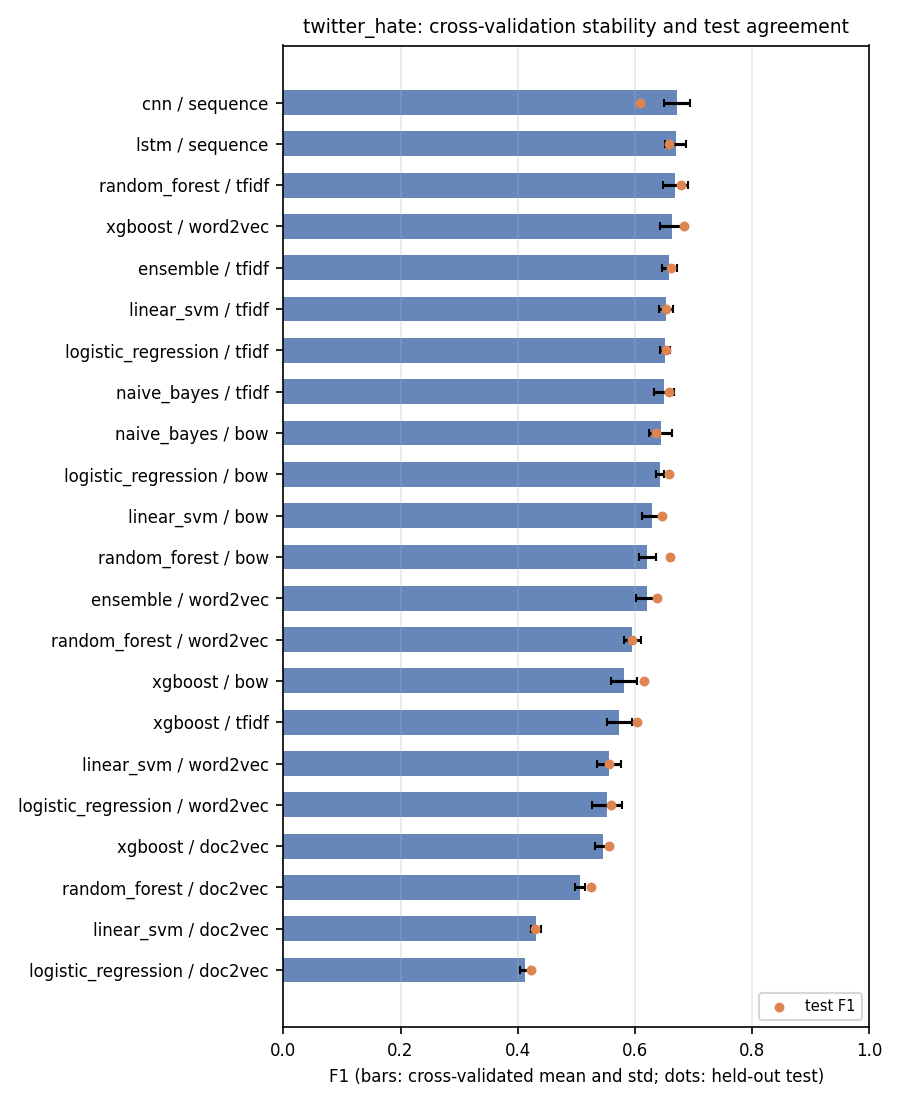
\includegraphics[width=\columnwidth]{cv_twitter_hate.png}
\caption{Hate corpus: cross-validated F1 (bars, with fold standard deviation) against test F1 (dots) for all 22 cells. Differences of 0.02 are within fold noise for most cells.}
\label{fig:cv}
\end{figure}

Fig.~\ref{fig:cv} places the differences in context: fold standard deviations are 0.01 to 0.02, so the top eight cells (cross-validated F1 0.650 to 0.672) are statistically indistinguishable on this corpus, and a claim that a network beats a linear model here would not survive the confidence intervals. Per-class scores of the selected models are given in Table~\ref{tab:perclass}: on the hate corpus the CNN at its tuned threshold trades recall (0.498) for precision (0.782) on the 448 positive test tweets.

\begin{table}[t]
\centering
\caption{Per-class test scores of the selected model on each dataset.}
\label{tab:perclass}
\begin{tabular}{llrccc}
\toprule
Dataset & Class & Support & Prec. & Rec. & F1 \\
\midrule
Hate & not hate & 5945 & 0.963 & 0.990 & 0.976 \\
 & hate & 448 & 0.782 & 0.498 & 0.608 \\
Vaccine & negative & 205 & 0.639 & 0.741 & 0.686 \\
 & neutral & 1172 & 0.930 & 0.861 & 0.894 \\
 & positive & 694 & 0.825 & 0.889 & 0.856 \\
IMDB & negative & 12500 & 0.895 & 0.866 & 0.880 \\
 & positive & 12500 & 0.870 & 0.898 & 0.884 \\
\bottomrule
\end{tabular}
\end{table}

\subsection{Representations}
\begin{table}[t]
\centering
\caption{Feature representations: best model per feature set and dataset (test F1, model in parentheses). Doc2Vec was not run on IMDB.}
\label{tab:features}
\begin{tabular}{llll}
\toprule
Features & Hate & Vaccine & IMDB \\
\midrule
counts & 0.636 (NB) & 0.775 (LR) & 0.856 (LR) \\
TF-IDF & 0.680 (RF) & 0.757 (Ens.) & 0.884 (SVM) \\
Word2Vec & 0.684 (XGB) & 0.552 (LR) & 0.846 (XGB) \\
Doc2Vec & 0.557 (XGB) & 0.475 (LR) & n/a \\
sequence & 0.608 (CNN) & 0.812 (CNN) & 0.876 (BiLSTM) \\
\bottomrule
\end{tabular}
\end{table}
Table~\ref{tab:features} confirms across all three corpora that sparse $n$-gram features are the strongest representation for classical learners: TF-IDF or counts give the best cell for every model except XGBoost, which reaches its best hate-speech score (0.684) on mean-pooled Word2Vec. Doc2Vec is the weakest representation for every model on both Twitter corpora (0.42 to 0.56 on hate, 0.42 to 0.48 on vaccine): with documents of ten to twenty tokens, inferred paragraph vectors carry little beyond noise, and linear models on them fall below naive Bayes on counts. Mean-pooled Word2Vec sits between the two; it helps tree models, which can exploit interactions between embedding dimensions, and hurts linear ones. On the vaccine corpus the gap is largest: embedding features reach 0.42 to 0.55 macro F1 against 0.70 to 0.78 for $n$-gram models, because the lexicon labeller responds to the presence of specific words that mean pooling blurs.

\subsection{Vaccine corpus}
The CNN is clearly ahead on the three-class task: macro F1 0.812 (cross-validated 0.799 \textpm{} 0.012, accuracy 0.859) against 0.775 for logistic regression on counts, 0.757 for the TF-IDF ensemble and for XGBoost on counts, and 0.779 for the BiLSTM. The per-class report (Table~\ref{tab:perclass}) shows the minority negative class (205 test tweets) at F1 0.686 with recall 0.741, the neutral majority at 0.894 and positive at 0.856. Because the target is the sign of a lexicon polarity, a model that captures short patterns around lexicon words (negation, intensifiers) reproduces the labeller better than a bag of words can; these numbers should be read as agreement with TextBlob, not as human-judged sentiment accuracy.

\subsection{IMDB}
On balanced, long documents the picture inverts. Logistic regression (F1 0.886, accuracy 0.885), the calibrated SVM (0.884, 0.882) and their ensemble with XGBoost (0.888, 0.885) on 20,000 TF-IDF terms are within 0.004 of each other with fold standard deviations of 0.002; the BiLSTM (0.876) and CNN (0.875) trained from scratch do not reach them, and the tree models trail by 0.02 to 0.03. The tuned thresholds of the best cells lie at 0.45 to 0.50, so thresholding is immaterial on this task. Accuracies of 88.2 to 88.5\,percent agree with the 88.9\,percent reported by Maas et al.~\cite{maas2011} for their learned word vectors with a linear classifier and sit below the 91.2\,percent of NB-SVM over bigrams~\cite{wang2012} and the 93\,percent and above of fine-tuned transformers~\cite{devlin2019}, which locates this grid precisely: it is the ceiling of models that train from scratch on a CPU in minutes.

\subsection{Cost}
\begin{table}[t]
\centering
\caption{Training cost of the best cell per model family: seconds to fit on the full training split (laptop CPU, 8 cores), hate-speech and IMDB tasks.}
\label{tab:cost}
\begin{tabular}{lrrrr}
\toprule
Model & \multicolumn{2}{c}{Hate} & \multicolumn{2}{c}{IMDB} \\
 & F1 & s & F1 & s \\
\midrule
Naive Bayes & 0.658 & 0.1 & 0.851 & 0.1 \\
Logistic regression & 0.654 & 0.1 & 0.886 & 0.1 \\
Linear SVM (calib.) & 0.654 & 0.2 & 0.884 & 0.3 \\
Random forest & 0.680 & 5.0 & 0.859 & 9.6 \\
XGBoost & 0.684 & 9.0 & 0.865 & 53.9 \\
Soft-voting ensemble & 0.662 & 3.2 & 0.888 & 45.1 \\
CNN & 0.608 & 22.7 & 0.875 & 86.4 \\
BiLSTM & 0.658 & 29.3 & 0.876 & 81.7 \\
\bottomrule
\end{tabular}
\end{table}
Table~\ref{tab:cost} reports the time to fit the best cell per family on the full training split. The linear models train in well under a second on tweets and under a second on reviews; the forest and XGBoost in seconds to tens of seconds; the networks in 20 to 30 seconds on tweets and 80 to 90 seconds on reviews. On the hate corpus the resulting differences in F1 are within one to two fold standard deviations; on IMDB the cheapest models are also the most accurate. Whether the 0.04 to 0.05 macro-F1 advantage of the CNN on the vaccine corpus is worth a hundredfold increase in training time and an uncalibrated score scale is an application decision that the benchmark makes explicit rather than hides.

\subsection{Comparison with the original study}
The thesis notebooks evaluated the same classical models on the hate corpus with the vectorizer fitted on training and test documents together and a fixed threshold of 0.3, reporting validation F1 between 0.51 and 0.66 for logistic regression, the SVM, the forest and XGBoost on count, TF-IDF and Word2Vec features (and far lower on Doc2Vec), a public-leaderboard F1 of 0.70 for tuned XGBoost on Word2Vec, and 94\,percent accuracy for naive Bayes on a split in which unlabelled test rows were assigned the negative class. Under the present protocol naive Bayes reaches F1 0.658 (accuracy 0.954, which is mostly the majority rate), XGBoost on Word2Vec 0.684 and the linear models 0.654: the ordering of the original study survives, its absolute numbers do not, and the one figure that looked best was an artefact of leakage and of reporting accuracy under imbalance.

\section{Threats to Validity}
\textbf{Weak labels.} The vaccine corpus is labelled by a lexicon; models are rewarded for learning its idiosyncrasies. The hate and IMDB corpora have human labels.
\textbf{Single test split.} Test scores come from one stratified holdout (the official split for IMDB). Cross-validated means and standard deviations are reported alongside, and we have avoided claims that are smaller than one standard deviation.
\textbf{Threshold transfer.} Thresholds selected on fold models are applied to refitted models; we quantified the cost (up to 0.064 F1 for the CNN) and identified cross-validation bagging as the remedy.
\textbf{Grid scope.} No pretrained language model is included; the grid characterises what training from scratch on a CPU achieves, and the IMDB comparison with the literature bounds the gap.
\textbf{Temporal validity.} Both Twitter corpora date from 2016 to 2021; vocabulary and hashtag usage have since moved, which is what the drift monitor in the released system is for.
\textbf{Hardware.} Timings are from one laptop and are indicative only.

\section{Conclusion}
We fixed one evaluation protocol and applied it to 56 combinations of corpus, representation and model. Three findings hold across the study. First, on imbalanced short text the ranking ability of classical and neural classifiers is nearly identical, and the reported differences in F1 are differences in calibration and threshold handling; tuning the threshold on out-of-fold predictions is worth up to 0.09 F1 for classical models and 0.14 for networks and must be part of any comparison, and over-confident networks transfer such thresholds worst. Second, sparse $n$-gram features remain the representation of choice for classical learners on short text, learned document embeddings are the weakest choice everywhere, and on balanced long documents linear models on TF-IDF match networks trained from scratch at a hundredth of the cost. Third, the numbers of the original notebook study were dominated by leakage and by accuracy under imbalance; a rigorous protocol preserves its ranking but not its figures. The released system makes these results regenerable from saved probabilities and keeps the selected models operable, with tracked runs, model cards, a database-backed prediction service and drift monitoring. Future work is cross-validation bagging of the neural cells, a fine-tuned transformer as an upper reference, and human annotation of a subset of the vaccine corpus to replace the lexicon labels.

\begin{thebibliography}{00}
\bibitem{pang2008} B. Pang and L. Lee, ``Opinion mining and sentiment analysis,'' \emph{Foundations and Trends in Information Retrieval}, vol. 2, no. 1-2, pp. 1-135, 2008.
\bibitem{liu2012} B. Liu, \emph{Sentiment Analysis and Opinion Mining}. San Rafael, CA, USA: Morgan \& Claypool, 2012.
\bibitem{go2009} A. Go, R. Bhayani, and L. Huang, ``Twitter sentiment classification using distant supervision,'' Stanford University, CS224N Project Report, 2009.
\bibitem{waseem2016} Z. Waseem and D. Hovy, ``Hateful symbols or hateful people? Predictive features for hate speech detection on Twitter,'' in \emph{Proc. NAACL Student Research Workshop}, San Diego, CA, USA, 2016, pp. 88-93.
\bibitem{davidson2017} T. Davidson, D. Warmsley, M. Macy, and I. Weber, ``Automated hate speech detection and the problem of offensive language,'' in \emph{Proc. 11th Int. AAAI Conf. Web and Social Media (ICWSM)}, Montreal, Canada, 2017, pp. 512-515.
\bibitem{mccallum1998} A. McCallum and K. Nigam, ``A comparison of event models for naive Bayes text classification,'' in \emph{Proc. AAAI Workshop on Learning for Text Categorization}, Madison, WI, USA, 1998, pp. 41-48.
\bibitem{joachims1998} T. Joachims, ``Text categorization with support vector machines: Learning with many relevant features,'' in \emph{Proc. 10th European Conf. Machine Learning (ECML)}, Chemnitz, Germany, 1998, pp. 137-142.
\bibitem{breiman2001} L. Breiman, ``Random forests,'' \emph{Machine Learning}, vol. 45, no. 1, pp. 5-32, 2001.
\bibitem{chen2016} T. Chen and C. Guestrin, ``XGBoost: A scalable tree boosting system,'' in \emph{Proc. 22nd ACM SIGKDD Int. Conf. Knowledge Discovery and Data Mining}, San Francisco, CA, USA, 2016, pp. 785-794.
\bibitem{wang2012} S. Wang and C. D. Manning, ``Baselines and bigrams: Simple, good sentiment and topic classification,'' in \emph{Proc. 50th Annu. Meeting Assoc. Computational Linguistics (ACL)}, Jeju Island, Korea, 2012, pp. 90-94.
\bibitem{maas2011} A. L. Maas, R. E. Daly, P. T. Pham, D. Huang, A. Y. Ng, and C. Potts, ``Learning word vectors for sentiment analysis,'' in \emph{Proc. 49th Annu. Meeting Assoc. Computational Linguistics (ACL)}, Portland, OR, USA, 2011, pp. 142-150.
\bibitem{mikolov2013} T. Mikolov, I. Sutskever, K. Chen, G. Corrado, and J. Dean, ``Distributed representations of words and phrases and their compositionality,'' in \emph{Advances in Neural Information Processing Systems 26}, Lake Tahoe, NV, USA, 2013, pp. 3111-3119.
\bibitem{le2014} Q. Le and T. Mikolov, ``Distributed representations of sentences and documents,'' in \emph{Proc. 31st Int. Conf. Machine Learning (ICML)}, Beijing, China, 2014, pp. 1188-1196.
\bibitem{kim2014} Y. Kim, ``Convolutional neural networks for sentence classification,'' in \emph{Proc. Conf. Empirical Methods in Natural Language Processing (EMNLP)}, Doha, Qatar, 2014, pp. 1746-1751.
\bibitem{hochreiter1997} S. Hochreiter and J. Schmidhuber, ``Long short-term memory,'' \emph{Neural Computation}, vol. 9, no. 8, pp. 1735-1780, 1997.
\bibitem{devlin2019} J. Devlin, M.-W. Chang, K. Lee, and K. Toutanova, ``BERT: Pre-training of deep bidirectional transformers for language understanding,'' in \emph{Proc. NAACL-HLT}, Minneapolis, MN, USA, 2019, pp. 4171-4186.
\bibitem{kaufman2012} S. Kaufman, S. Rosset, C. Perlich, and O. Stitelman, ``Leakage in data mining: Formulation, detection, and avoidance,'' \emph{ACM Trans. Knowledge Discovery from Data}, vol. 6, no. 4, art. 15, 2012.
\bibitem{cawley2010} G. C. Cawley and N. L. C. Talbot, ``On over-fitting in model selection and subsequent selection bias in performance evaluation,'' \emph{J. Machine Learning Research}, vol. 11, pp. 2079-2107, 2010.
\bibitem{lipton2014} Z. C. Lipton, C. Elkan, and B. Naryanaswamy, ``Optimal thresholding of classifiers to maximize F1 measure,'' in \emph{Proc. ECML PKDD}, Nancy, France, 2014, pp. 225-239.
\bibitem{platt1999} J. C. Platt, ``Probabilistic outputs for support vector machines and comparisons to regularized likelihood methods,'' in \emph{Advances in Large Margin Classifiers}, A. J. Smola, P. Bartlett, B. Sch\"olkopf, and D. Schuurmans, Eds. Cambridge, MA, USA: MIT Press, 1999, pp. 61-74.
\bibitem{niculescu2005} A. Niculescu-Mizil and R. Caruana, ``Predicting good probabilities with supervised learning,'' in \emph{Proc. 22nd Int. Conf. Machine Learning (ICML)}, Bonn, Germany, 2005, pp. 625-632.
\bibitem{guo2017} C. Guo, G. Pleiss, Y. Sun, and K. Q. Weinberger, ``On calibration of modern neural networks,'' in \emph{Proc. 34th Int. Conf. Machine Learning (ICML)}, Sydney, Australia, 2017, pp. 1321-1330.
\bibitem{davis2006} J. Davis and M. Goadrich, ``The relationship between precision-recall and ROC curves,'' in \emph{Proc. 23rd Int. Conf. Machine Learning (ICML)}, Pittsburgh, PA, USA, 2006, pp. 233-240.
\bibitem{pedregosa2011} F. Pedregosa et al., ``Scikit-learn: Machine learning in Python,'' \emph{J. Machine Learning Research}, vol. 12, pp. 2825-2830, 2011.
\bibitem{paszke2019} A. Paszke et al., ``PyTorch: An imperative style, high-performance deep learning library,'' in \emph{Advances in Neural Information Processing Systems 32}, Vancouver, Canada, 2019, pp. 8024-8035.
\bibitem{loria2018} S. Loria, ``TextBlob: Simplified text processing,'' software, release 0.15, 2018. [Online]. Available: \url{https://textblob.readthedocs.io}
\bibitem{sculley2015} D. Sculley et al., ``Hidden technical debt in machine learning systems,'' in \emph{Advances in Neural Information Processing Systems 28}, Montreal, Canada, 2015, pp. 2503-2511.
\bibitem{mitchell2019} M. Mitchell et al., ``Model cards for model reporting,'' in \emph{Proc. Conf. Fairness, Accountability, and Transparency (FAT*)}, Atlanta, GA, USA, 2019, pp. 220-229.
\bibitem{zaharia2018} M. Zaharia et al., ``Accelerating the machine learning lifecycle with MLflow,'' \emph{IEEE Data Engineering Bulletin}, vol. 41, no. 4, pp. 39-45, 2018.
\bibitem{siddiqi2006} N. Siddiqi, \emph{Credit Risk Scorecards: Developing and Implementing Intelligent Credit Scoring}. Hoboken, NJ, USA: Wiley, 2006.
\end{thebibliography}

\end{document}
